\documentclass[a4paper, 12pt]{article}
\usepackage[english]{babel}
\usepackage[pdftex]{graphicx}
\usepackage[pdftex,dvipsnames]{xcolor}  % Coloured text etc.
\usepackage[T1]{fontenc}
\usepackage{wrapfig}
\usepackage{graphicx} 
\usepackage{algpseudocode}
\usepackage{algorithm}
\usepackage{minted}
\usepackage{hyperref}
\usepackage{csquotes}
\usepackage{biblatex} %Imports biblatex package
\addbibresource{Citations.bib} %Import the bibliography file
\usepackage{amssymb}
\usepackage{tikz}
\usepackage{caption}
\usepackage{subcaption}
\usepackage{hyphenat}
\usepackage{siunitx}
\usepackage{changepage}   % for the adjustwidth environment
\usepackage[toc,page]{appendix}
\usepackage[inkscapelatex=true]{svg}

\setlength {\marginparwidth }{2cm}
\usepackage[colorinlistoftodos,prependcaption,textsize=tiny]{todonotes}
\usepackage{xargs}


\hfuzz 40pt
\newenvironment{tab}{\begin{adjustwidth}{1cm}{1cm} \itshape }{ \end{adjustwidth}}
\newcommandx{\unsure}[2][1=]{\todo[linecolor=red,backgroundcolor=red!25,bordercolor=red,#1]{#2}}
\newcommandx{\change}[2][1=]{\todo[linecolor=blue,backgroundcolor=blue!25,bordercolor=blue,#1]{#2}}
\newcommandx{\info}[2][1=]{\todo[linecolor=OliveGreen,backgroundcolor=OliveGreen!25,bordercolor=OliveGreen,#1]{#2}}
\newcommandx{\improvement}[2][1=]{\todo[linecolor=Plum,backgroundcolor=Plum!25,bordercolor=Plum,#1]{#2}}
\newcommandx{\thiswillnotshow}[2][1=]{\todo[disable,#1]{#2}}

\begin{document}
\begin{titlepage}
\begin{center}
{\Large University of Mons}\\[1ex]
{\Large Sciences Faculty}\\[1ex]
{\Large Computer Science Department}\\[2.5cm]

\newcommand{\HRule}{\rule{\linewidth}{0.3mm}}
% Title
\HRule \\[0.3cm]
{ \LARGE \bfseries LoRa frame detection and capture \\[0.3cm]}
{ \LARGE \bfseries Internship Report \\[0.1cm]} 
\HRule \\[1.5cm]

% Author and supervisor
\begin{minipage}[t]{0.45\textwidth}
\begin{flushleft} \large
\emph{Head of Service :}\\
Bruno \textsc{Quoitin}\\[3mm]
\emph{Supervisor :}\\
Aqeel \textsc{Ahmed}\\
\end{flushleft}
\end{minipage}
\begin{minipage}[t]{0.45\textwidth}
\begin{flushright} \large
\emph{Author :} \\
Maxime \textsc{Bartha}\\
\end{flushright}
\end{minipage}\\[2ex]

\vfill

% Bottom of the page
\begin{center}
\begin{tabular}[t]{c c c}

\includegraphics[height=1.5cm]{images/logoumons.jpg} &
\hspace{0.3cm} &

\includegraphics[height=1.5cm]{images/logofs.jpg}
\end{tabular}
\end{center}~\\
 
{\large Academic Year 2024-2025}

\end{center}
\end{titlepage}

\tableofcontents
\newpage

% ------------------------------------------
%       Formating rules : 
%
% ------------------------------------------

\section{Introduction}
This report is a follow-up of an internship realized during the summer of 2025. 
This internship is part of a University program for third year students to have an introduction to research at Umons.\\
To this end, a student follows a PhD student and assists them in their work.

In my case, the PhD student supervising this internship is Aqeel Ahmed.
His PhD is about Radio Frequency Fingerprinting (RFFI) of LoRa IQ signals using Deep Learning (DL) algorithms.\\
In a recent survey \cite{AqeelSurvey}, he describes fingerprints as :
\begin{tab}
  The entangled features of electronic hardware originating from the manufacturing process.
\end{tab}
\noindent
He then describes RFFI as : 
\begin{tab}
  The process of extracting those features from the radio signal
  of the device with hardware imperfections that make the transmitter distinguishable among
  others even if they are from the same model and manufacturer \cite{7902125}.
\end{tab}
Aqeel, in the same survey \cite{AqeelSurvey}, notes the lack of available data for LoRa RFFI. \\
Due to this lack of databases, which is needed for DL model training, the creation of them is an important subject leading us to the objective of this internship.  

\subsection{Objective}
The objective of this internship is to assist Aqeel in the collection of new LoRa IQ samples to experiment with Radio Fingerprinting classification with deep learning models.
To this end, the collected samples are coming from multiples LoRa capable devices and labelled per device and time. 
Those captures are to be well classified and shouldn't take too long to make. 

\subsection{Overview}
Section \ref{LoraBasics} explains the basic knowledge required to understand LoRa related discussions in this report.\\
Section \ref{Methodo} presents the material used, the structure of experiments as well as the different scenarios tested. A discussion on the possible implementations and transmission strategy is also made to assess the most reliable method.\\
A description of the selected implementation is made in section \ref{Impl}.\\
The results and their quality are assessed and discussed in section \ref{Res}.\\
Finally, in section \ref{conclu}, propositions of improvements are presented and the conclusion of this work is done.

\section{LoRa Basics}\label{LoraBasics}
In this section, the essentials of the LoRA modulation technique (section \ref{CSS}), preamble format (section \ref{preamble}) and demodulation technique (section \ref{demod}) are discussed to understand their uses in the experiments.

\subsection{Chirp Spread Spectrum modulation}\label{CSS}
LoRa is a long-range, low-power, proprietary radio interface.
It is based on a Chirp Spread Spectrum (CSS) modulation technique. 
The basic element of this technique is called a chirp. 
A chirp is a sinusoidal signal whose frequency varies linearly over time. 
Details on the underlying math can be found in a recent article \cite{CSSTuto} explaining CSS modulation and the key advances made to understand it.
To understand the experiments made in this paper, only the frequency domain is explored and explained.

There are three necessary parameters for LoRa communication : a carrier frequency ($F_c$), a bandwidth ($B$) and spreading factor ($SF$).\\
The carrier frequency of the signal is set in Europe as \qty{868}{\mega\hertz}.
Finally, the spreading factor represents the number of bits carried in a LoRa symbol. For example, with an SF of 7, a LoRa symbol can represent a value ranging from 0 to $2^7 -1 = 127$.

LoRa symbols are chrips whose duration $T$ depends on the bandwidth $B$ and spreading factor $SF$ as the equation \ref{eq:symbolDuration} shows. 
\begin{equation}
  T = \frac{2^{SF}}{B} 
  \label{eq:symbolDuration}
\end{equation}
A LoRa symbol frequency varies from $F_c - B/2$ to $F_c + B/2$ linearly as shown in the Figure \ref{chirps.symb}. It implies that when a signal reaches a frequency of $F_c + B/2$ (resp. $F_c -B/2$), wraps up to $F_c - B/2$ (resp. $F_c + B/2$) before varying linearly again.

\begin{figure}[ht]
  \centering
  \hspace{-1.5cm}
  \begin{subfigure}[ht]{0.51\textwidth}
    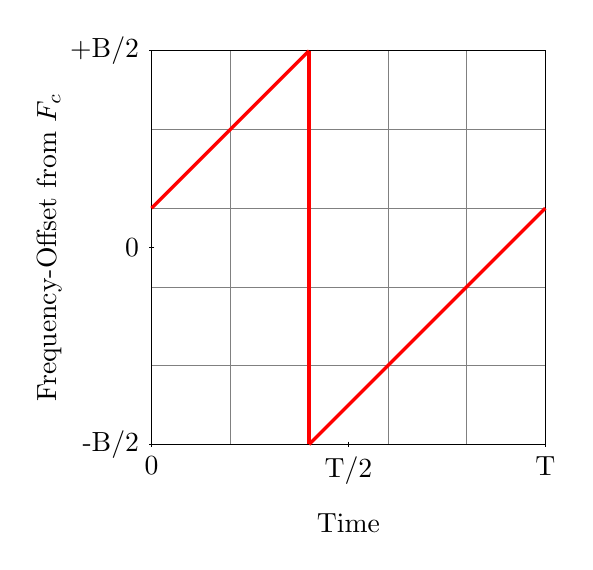
\begin{tikzpicture}
    \draw[step=1cm,gray,very thin] (0,0) grid (5,5);
    \draw (0,0) -- (5,0) -- (5,5) -- (0,5) -- (0,0);
    \node at (-1.3,2.5) [rotate=90]  {Frequency-Offset from $F_c$};
    \node at (2.5,-1) {Time};

    \draw (0,1pt) -- (0, -1pt) node [anchor=north] {0};
    \draw (2.5cm,1pt) -- (2.5cm, -1pt) node [anchor=north] {T/2};
    \draw (5cm,1pt) -- (5cm, -1pt) node [anchor=north] {T};

    \draw (1pt, 0cm) -- (-1pt, 0cm) node [anchor=east] {-B/2};
    \draw (1pt, 2.5cm) -- (-1pt, 2.5cm) node [anchor=east] {0};
    \draw (1pt, 5cm) -- (-1pt, 5cm) node [anchor=east] {+B/2};

    \draw (0,3) -- (2,5) [color=red, very thick];
    \draw (2,5) -- (2,0) [color=red, very thick];
    \draw (2,0) -- (5,3) [color=red, very thick];
    \end{tikzpicture}
    \caption{LoRa Symbol}
    \label{chirps.symb}
  \end{subfigure}
  \begin{subfigure}[ht]{0.51\textwidth}
    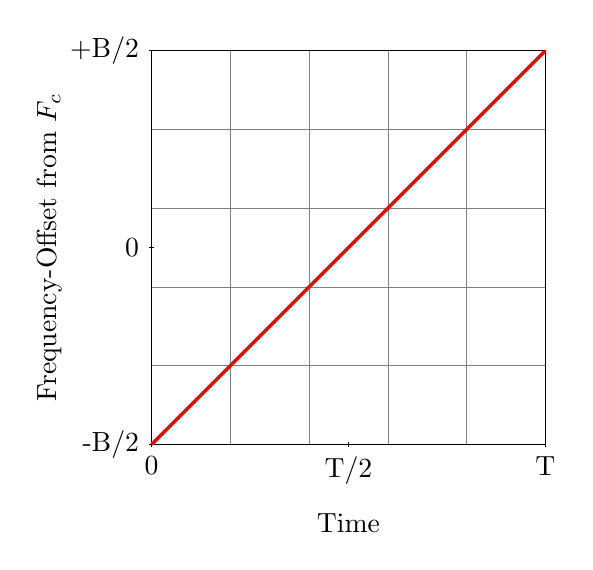
\begin{tikzpicture}
    \draw[step=1cm,gray,very thin] (0,0) grid (5,5);
    \draw (0,0) -- (5,0) -- (5,5) -- (0,5) -- (0,0);
    \node at (-1.3,2.5) [rotate=90]  {Frequency-Offset from $F_c$};
    \node at (2.5,-1) {Time};
    \draw (0,1pt) -- (0, -1pt) node [anchor=north] {0};
    \draw (2.5cm,1pt) -- (2.5cm, -1pt) node [anchor=north] {T/2};
    \draw (5cm,1pt) -- (5cm, -1pt) node [anchor=north] {T};

    \draw (1pt, 0cm) -- (-1pt, 0cm) node [anchor=east] {-B/2};
    \draw (1pt, 2.5cm) -- (-1pt, 2.5cm) node [anchor=east] {0};
    \draw (1pt, 5cm) -- (-1pt, 5cm) node [anchor=east] {+B/2};

    \draw (0,0) -- (5,5) [color=red, very thick];
    \end{tikzpicture}
    \caption{baseup chirp}
    \label{chirps.base-upchirp}
  \end{subfigure}
  \caption{Chirps of duration $T$ and bandwidth $B$ in the frequency domain (frequency with respect to time). The frequency axis is relative to the carrier frequency $F_c$.}
  \label{chirps}
\end{figure}

The value represented depends on the start (and final) frequency of the LoRa symbol.
For a symbol of value s, the starting frequency $f_0 = F_c - B/2 + \frac{sB}{2^{SF}}$.
Intuitively, the value is represented by the "frequency phase" of the received signal.  
It is possible to observe that the symbol represented in Figure \ref{chirps.base-upchirp} is a baseup chirp because its starting frequency is $F_c - B/2$.\\
A baseup chirp represents a value of 0 and varies from $F_c - B/2$ to $F_c + B/2$. Similarly, a base-down chirp starts at $F_c + B/2$ and ends at $F_c - B/2$, decreasing linearly rather than increasing.

\subsection{Preamble}\label{preamble}
A LoRa frame is composed of 3 parts: the preamble part, the Start of Frame Delimiter (SFD) and the actual data symbols.
The preamble part is composed of 8 or more baseup chirps and a sync word part composed of two symbols.
The SFD is composed of 2.25 base-down chirps. 

A captured representation of a preamble + SFD can be seen in Figure \ref{fig:wholePream}.

\begin{figure}[ht]
  \begin{center}
    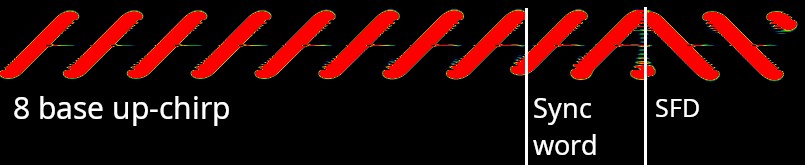
\includegraphics[width=0.95\textwidth]{images/LoRaPreambleWithText.png}
  \end{center}
  \caption[test 12]{Spectrogram of a captured LoRa preamble and SFD from inspectrum\footnotemark}\label{fig:wholePream}
\end{figure}
\footnotetext{inspectrum is an open source radio signal analyser. Its source code can be found at \url{https://github.com/miek/inspectrum}} 

The data symbols part isn't discussed because only the preamble and SFD parts are used for the deep learning algorithms.
By taking more of the frame, for example the header, the DL model is capable of detecting features not specific to hardware impairments.  
The preamble and SFD part forms a small stable set of symbols only impacted by hardware impairments.


\subsection{Demodulation}\label{demod}
The demodulation technique used in the experiments comes from a comprehensive paper named \textit{From Demodulation to Decoding} \cite{demToDec}. The method proposed can be described in 4 steps graphically explained in Figure \ref{fig:demToD}.

i. Retrieve the sampled data containing a LoRa symbol with a sampling frequency $f_{samp}$ of at least two times the bandwidth $Bw$.

ii. Multiply the retrieved signal, of initial frequency $f_0$, with a base downchirp to obtain two constant signals with frequency $f_0$ and $f_0 -Bw$.

iii. Apply a Fast Fourier Transform (FFT) on the result of the multiplication. This gives two distinct peaks at $f_0$ and $f_{samp} - Bw + f_0$ as shown in Figure \ref{fig:demToD}(iii).

iv. The paper then proposes two options to merge those peaks. A Fine-Grained Phase Alignment (FPA) and a Coarse-grained Phase Alignment. CPA is much less computationally heavy than FPA and has marginally worst results.
In either case, the result gives an FFT peak at $f_0$.


\begin{figure}[ht]
  \begin{center}
    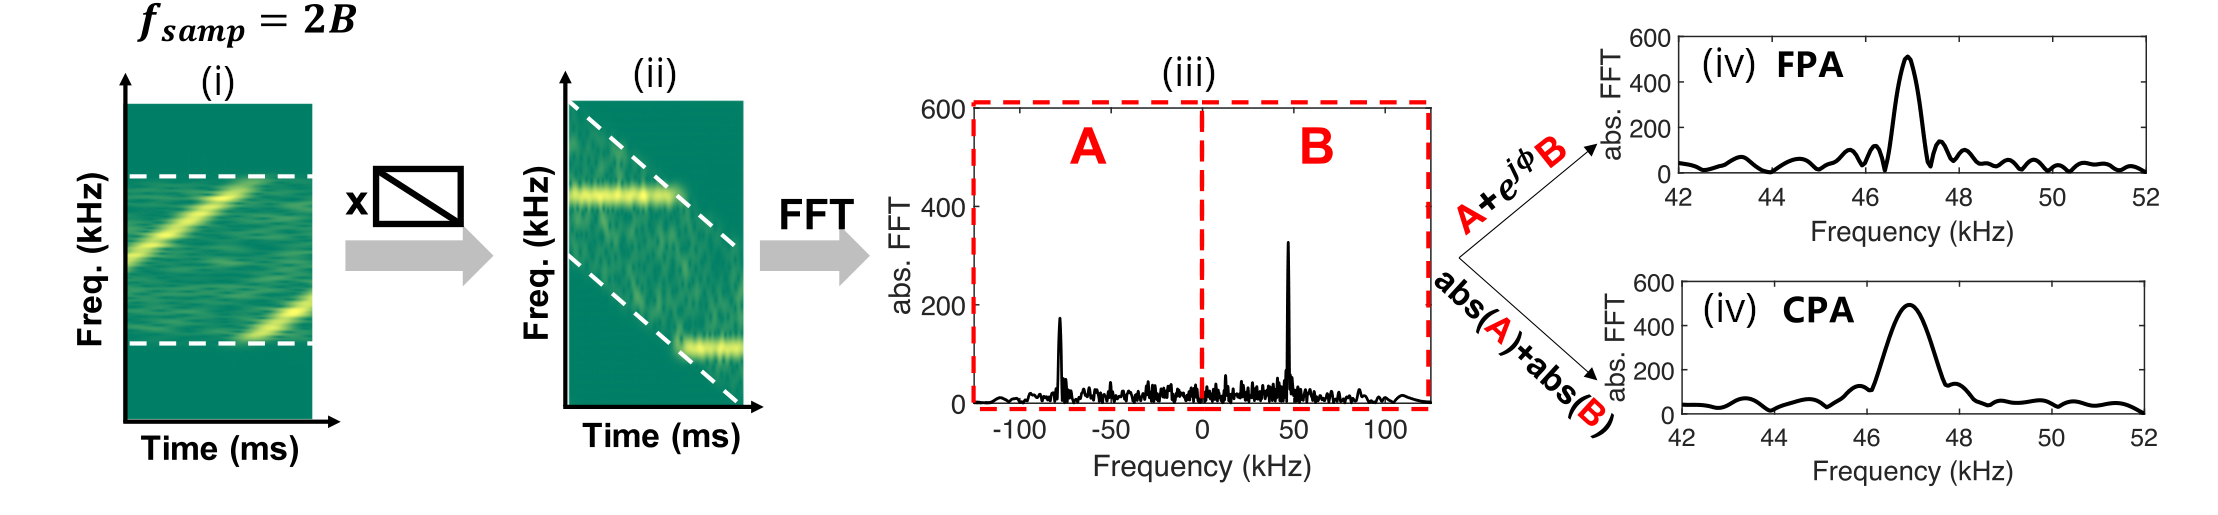
\includegraphics[width=0.95\textwidth]{images/demodSteps.png}
  \end{center}
  \caption{Graphical explanation used in the reference paper \cite{demToDec}.}\label{fig:demToD}
\end{figure}

\section{Methodology}\label{Methodo}

\todo[inline]{Present the following section once they are finished}

\subsection{Material}
The use of material in our experiments can be separated into two parts :

\textbf{The receiver Part} uses a laptop, an USRP \unsure{ unsure of the exact model (B210 or B200)} B2?0 Software Defined Radio (SDR) with the enclosure kit and an \unsure{which brand} antenna.

\textbf{The transmitter Part} uses a laptop, 4 StarTech USB hubs (ST7200USBM), 20 Arduino MKR1310 devices, a Velleman 5V lab power supply (LABPS3005SM), soldered copper wires to supply the Arduino devices and a handmade frame to attach the Arduino devices to. 

\improvement[inline]{Refer to the transmitter appendix to show the handmade frame}

\subsection{Ls.ayout of the experiments}
First, the singular setups of the receiver and transmitter part are discussed then the overall layout is presented.

\textbf{The receiver setup} is straight forward : the laptop is connected to the USRP SDR by USB. The SDR antenna is vertical. The Figure \ref{fig:receiverSheme} shows a schematic of the receiver setup.

\begin{figure}
  \begin{center}
    \includesvg[height=0.17\textheight]{images/receiverSheme.svg}
  \end{center}
  \caption{Receiver side schematic. The receiver laptop is connected to the USRP by USB. The SDR captures signals through its antenna.}\label{fig:receiverSheme}
\end{figure}

\improvement[inline]{photo of the Receiver part in appendix}

\newpage
\textbf{The transmitter setup} is more complex :
the laptop is connected to a first USB HUB on which the 3 other USB hubs are connected to form a star topology. The choice of such a topology is to flatten the USB communication with all 20 Arduino devices.
The Arduino devices are connected to the outermost USB hubs and powered externally by the lab power supply through their back pins with the soldered cables. The power supply is programmed with \qty{5}{\volt} of tension and \qty{1}{\ampere} of current.\\  
The Figure \ref{fig:transConn} shows the USB connections from the laptop to the Arduino devices.
Figure \ref{fig:transPower} shows the power supply schematic of the transmitter side. 


\improvement[inline]{photo of the transmitter part in appendix}


\begin{figure}[H]
  \begin{center}
    \includesvg[width=0.999\textwidth]{images/transmitterConnections.svg}
  \end{center}
  \caption{Receiver side USB connections schematic. The transmitter laptop is connected to the top level USB HUB on which the outermost hub are connected. Twenty devices with antennas are then connected to the outermost hubs.}\label{fig:transConn}
\end{figure}

\begin{figure}[ht]
  \begin{center}
    \includesvg[width=0.90\textwidth]{images/TransPower.svg}
  \end{center}
  \caption{Receiver side power supply schematic. The composition is as follows : five sets of devices are connected in parallel to the lab power supply. In a set all devices are connected in series through their back pins (VIN and GND).}\label{fig:transPower}
\end{figure}

\subsection{Software}
The method to transmit and receive frame is discussed with two possible proposed methods :

\textbf{Round-robin method} : 

\textbf{One by One method} : 



\subsection{Scenarios} 
The scenarios of capture are to be 



\section{Implementation}\label{Impl}
\section{Results}\label{Res}





\section{Conclusion}\label{conclu}


\subsection{Possible improvements}
Presenting the issues still in place and give an idea on how we might be able to fix them
\printbibliography

\newpage
\begin{appendices}

\section{First appendix}
\section{Second appendix}
  
\end{appendices}

\listoftodos[Notes]

\end{document}
